\documentclass[10pt]{jhwhw}
\author{Ian Malerich}
\title{Math S 373: Homework 1}
\usepackage{amssymb, amsfonts, amsmath, mathtools, graphicx, breqn, soul}
\usepackage{minted, subfig, float, scrextend, setspace, amsthm}
\usemintedstyle{friendly}

\begin{document}
\raggedright

%% Problem 1
\problem{} (10 points)
	Find the least squares polynomial of degree 2 for the data in the following
	table. Compute the error E. Graph the data and the polynomial.
	\bigbreak
	\begin{tabular}{ccccccc}
		\hline
		$x_i$ & 1.0 & 1.1 & 1.3 & 1.5 & 1.9 & 2.1 \\
		$y_i$ & 1.84 & 1.96 & 2.21 & 2.45 & 2.94 & 3.18 \\
		\hline
	\end{tabular}

\solution

	A = 
	\left[\begin{array}{ccc}
		1 & 1 & 1 \\
		1 & 1.1 & 1.1^2 \\
		1 & 1.3 & 1.3^2 \\
		1 & 1.5 & 1.5^2 \\
		1 & 1.9 & 1.9^2 \\
		1 & 2.1 & 2.1^2 \\
	\end{array} \right]
	b = 
	\left[\begin{array}{c}
		1.84 \\ 1.96 \\ 2.21 \\ 2.45 \\ 2.94 \\ 3.18 \\
	\end{array} \right]

	\bigbreak
	$A^TAa = A^Tb \Rightarrow (A^TA)^{-1}(A^TA)a = (A^TA)^{-1}A^Tb \Rightarrow
	a = (A^TA)^{-1}A^Tb$

	\begin{align*}
	a &= 
	\left[\begin{array}{ccc}
		66.841 & -90.719 & 28.748 \\
		-90.719 & 124.544 & -39.811 \\
		28.748 & -39.811 & 12.832 \\
	\end{array} \right]
	\left[\begin{array}{ccc}
		1 & 1 & 1 & 1 & 1 & 1 \\
		1 & 1.1 & 1.3 & 1.5 & 1.9 & 2.1 \\
		1 & 1.21 & 1.69 & 2.25 & 3.61 & 4.41 \\
	\end{array} \right]
	\left[\begin{array}{c}
		1.84 \\ 1.96 \\ 2.21 \\ 2.45 \\ 2.94 \\ 3.18 \\
	\end{array} \right]
	\\ &= 
	\left[\begin{array}{cccccc}
		4.86939 & 1.83451 & -2.51039 & -4.55547 & -1.74620 & 3.10816 \\
		-5.98639 & -1.89239 & 3.90693 & 6.52134 & 2.19542 & -4.74490 \\
		1.76871 & 0.48237 & -1.32035 & -2.09647 & -0.56895 & 1.773469 \\
	\end{array} \right]
	\left[\begin{array}{c}
		1.84 \\ 1.96 \\ 2.21 \\ 2.45 \\ 2.94 \\ 3.18 \\
	\end{array} \right]
	\\ &= 
	\left[\begin{array}{c}
		0.596581 \\ 1.253293 \\ -0.010853 \\
	\end{array} \right]
	\end{align*}

	This gives us the interpolating polynomial as
	$
		P_2(x) = -0.010853x^2 + 1.253293x + 0.596581
	$.

	Evaluating our initial points using our polynomial produces the results...
	\bigbreak
	\begin{tabular}{ccccccc}
		\hline
		$x_i$ & 1.0 & 1.1 & 1.3 & 1.5 & 1.9 & 2.1 \\
		$y_i$ & 1.84 & 1.96 & 2.21 & 2.45 & 2.94 & 3.18 \\
		$P(x_i)$ & 1.839 & 1.9621 & 2.2075 & 2.4521 & 2.9387 & 3.1806 \\
		$|P(x_i)-y_i|$ & -9.79e-4 & 2.0712e-3 & 2.4797e-3 & 2.1012e-3 & 1.3416e-3 & 6.3457e-4 \\
		\hline
	\end{tabular} \bigbreak
	Taking the sum of the differences finds the total error across all interpolating
	points as $E = 6.69\times 10^{-6}$.

	\bigbreak
	We can see that the least squares fit finds a polynomial which is 
	almost linear, but not quite. From both the graph below, and the error above,
	the polynomial is clearly doing a good job (though not perfect) of fitting to
	the points.
	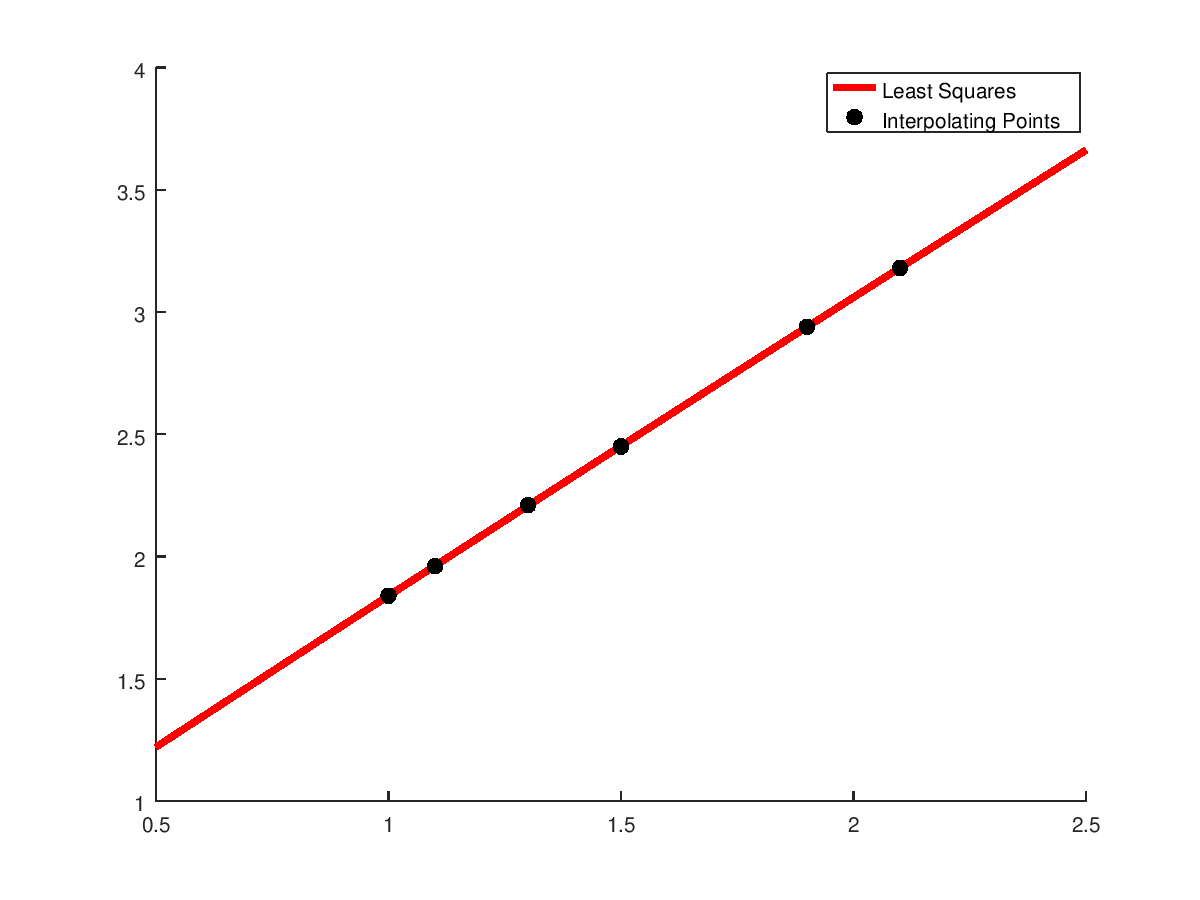
\includegraphics[scale=0.75]{p1}

%% Problem 2
\problem{} (20 points)

	\begin{enumerate}
		\item Find the least squares polynomial of degree 2 for the following function
			$f(x)$ on the indicated interval
			$$
				f(x) = e^x,\ [-1,1]
			$$
			Compute the error E. Graph the function and the polynomial.
		\item Repeat (a) with Legendre Polynomials.
	\end{enumerate}

\solution

	\part
	I will be using the $x=(-1,0,1)$ as interpolating points to 
	find my least squares polynomial, thus we want to use the following matrices
	in our system.

	\bigbreak
	$
	A = 
	\left[\begin{array}{ccc}
		1 & -1 & 1 \\
		1 & 0 & 0 \\
		1 & 1 & 1 \\
	\end{array} \right]
	b = 
	\left[\begin{array}{c}
		\frac{1}{e} & 1 & e \\
	\end{array} \right]
	$
	\bigbreak
	$A^TAa = A^Tb \Rightarrow (A^TA)^{-1}(A^TA)a = (A^TA)^{-1}A^Tb \Rightarrow
	a = (A^TA)^{-1}A^Tb$

	\bigbreak
	\begin{align*}
		a &= 
		\left[\begin{array}{ccc}
			1 & 0 & -1 \\
			0 & 0.5 & 0 \\
			-1 & 0 & 1.5 \\
		\end{array} \right]
		\left[\begin{array}{ccc}
			1 & 1 & 1 \\
			-1 & 0 & 1 \\
			1 & 0 & 1 \\
		\end{array} \right]
		\left[\begin{array}{c}
			\frac{1}{e} & 1 & e \\
		\end{array} \right]
		\\ &= 
		\left[\begin{array}{ccc}
			0 & 1 & 0 \\
			-0.5 & 0 & 0.5 \\
			0.5 & -1 & 0.5 \\
		\end{array} \right]
		\left[\begin{array}{c}
			\frac{1}{e} & 1 & e \\
		\end{array} \right]
		\\ &=
		\left[\begin{array}{c}
			1 \\ 1.7520 \\ 0.54308
		\end{array} \right]
	\end{align*}
	\bigbreak
	This gives us the interpolating polynomial $P_2(x) = 0.54308x^2 + 1.17520x + 1$.
	Evaluating our initial points using our polynomial produces the results\ldots

	\bigbreak
	\begin{tabular}{cccc}
		\hline
		$x_i$ & -1.0 & 0 & 1.0 \\
		$y_i$ & $\frac{1}{e}$ & 1 & e \\
		$P(x_i)$ & 0.36788 & 1.0 & 2.71828 \\
		$|P(x_i)-y_i|$ & 5.5883e-7 & 0 & 1.8285e-6 \\
		\hline
	\end{tabular}
	\bigbreak
	Taking the sum of the differences finds the total error across all interpolating
	points as $E = 2.3873\times 10^{-6}$.
	If we look over the range $[-1, 1]$ and want to compute the total error 
	(not just the interpolating points), we simply compute
	$\int_{-1}^1 |P(x) - e^x|dx = 0.0890387$.
	
	\bigbreak
	From the graph below, we can see that the interpolating polynomial closely matches,
	but diverges slightly from $e^x$. Notably, the polynomial switches from 
	underestimating to overestimating after crossing $x=0$.
	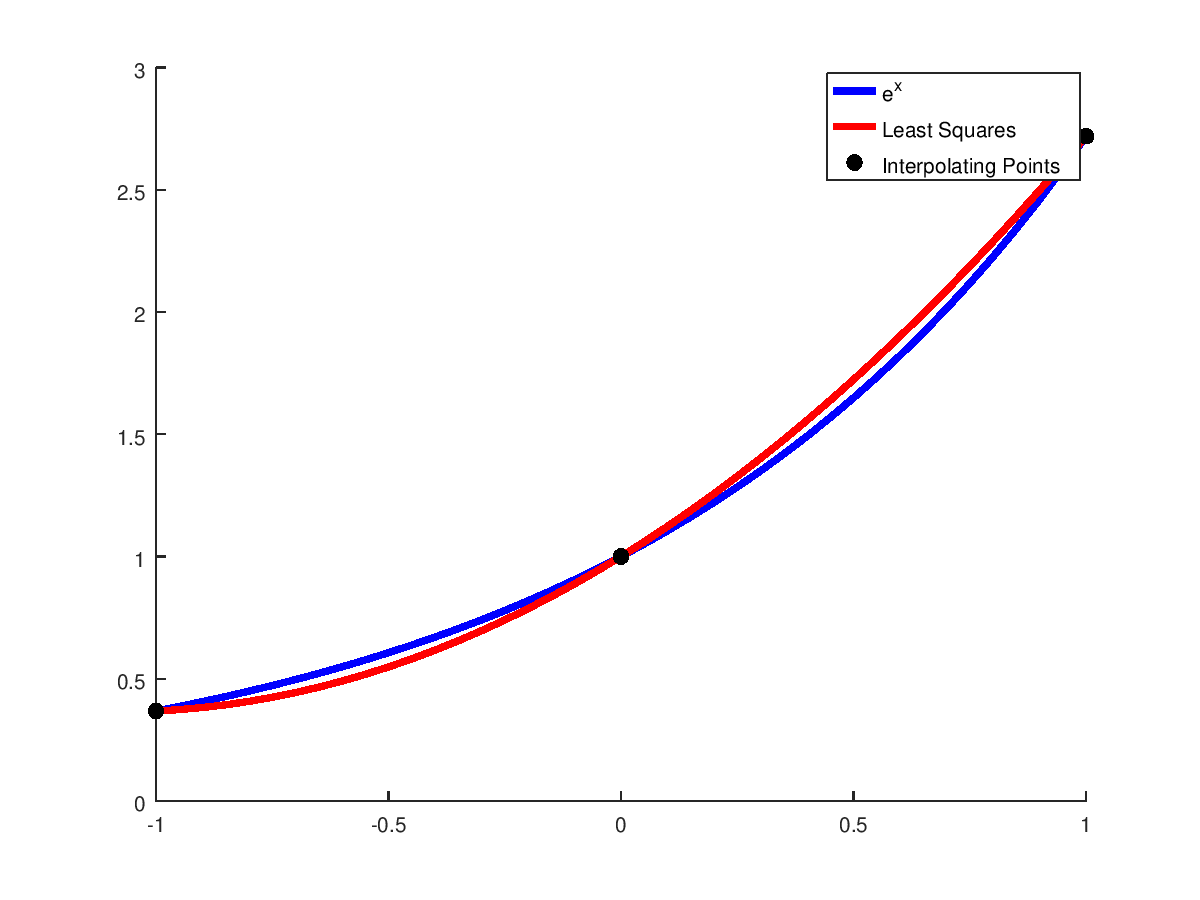
\includegraphics[scale=0.75]{p2}

	\part

	$b = 
	\left[\begin{array}{c}
		\int_{-1}^1 e^x P_0(x) dx \\
		\int_{-1}^1 e^x P_1(x) dx \\
		\int_{-1}^1 e^x P_2(x) dx \\
	\end{array} \right] =
	\left[\begin{array}{c}
		\int_{-1}^1 e^x dx \\
		\int_{-1}^1 e^x x dx \\
		\int_{-1}^1 e^x \frac{1}{2}(3x^2-1) dx \\
	\end{array} \right] =
	\left[\begin{array}{c}
		e - \frac{1}{e} \\
		\frac{2}{e} \\
		0.143126 \\
	\end{array} \right] =
	\left[\begin{array}{c}
		2.3504 \\
		0.73576 \\
		0.143126 \\
	\end{array} \right]
	$
	\bigbreak
	$d = 
	\left[\begin{array}{c}
		\frac{2(1)-1}{2}b_1 \\
		\frac{2(2)-1}{2}b_2 \\
		\frac{2(3)-1}{2}b_3 \\
	\end{array} \right] =
	\left[\begin{array}{c}
		\frac{1}{2}\times 2.3504 \\
		\frac{3}{2}\times 0.73576 \\
		\frac{5}{2}\times 0.143126 \\
	\end{array} \right] =
	\left[\begin{array}{c}
		1.1752 \\
		1.1036 \\
		0.35781 \\
	\end{array} \right]
	$
	\bigbreak
	The Legendre Polynomial Approximation is then given by\ldots
	\begin{align*}
		1.1752P_0 + 1.1036P_1 + 0.35781P_2 &=
		1.1752 + 1.1036x + 0.35781\frac{1}{2}(3x^2-1)  \\
		&= 0.536715x^2 + 1.1036x + 0.996295 \\
	\end{align*}

	\clearpage
	We can compute error over the bounds by taking $\integral_{-1}^1 |L_2(x) - e^x|dx
	= 0.0458856$. Recall the error for least squares was $0.0890387$, so we have 
	approximately halved our error despite both polynomials having degree 2. Note that
	we may have found a better least squares polynomial if we had used different
	interpolating points, these were not necessary for the Legendre approximation.

	\bigbreak
	Below we can visually confirm that this polynomial is doing a decent job
	of approximating $e^x$ on our given bounds. It appears to be more consistent
	and accurate than the least squares polynomial 
	but with greater error towards the end points.
	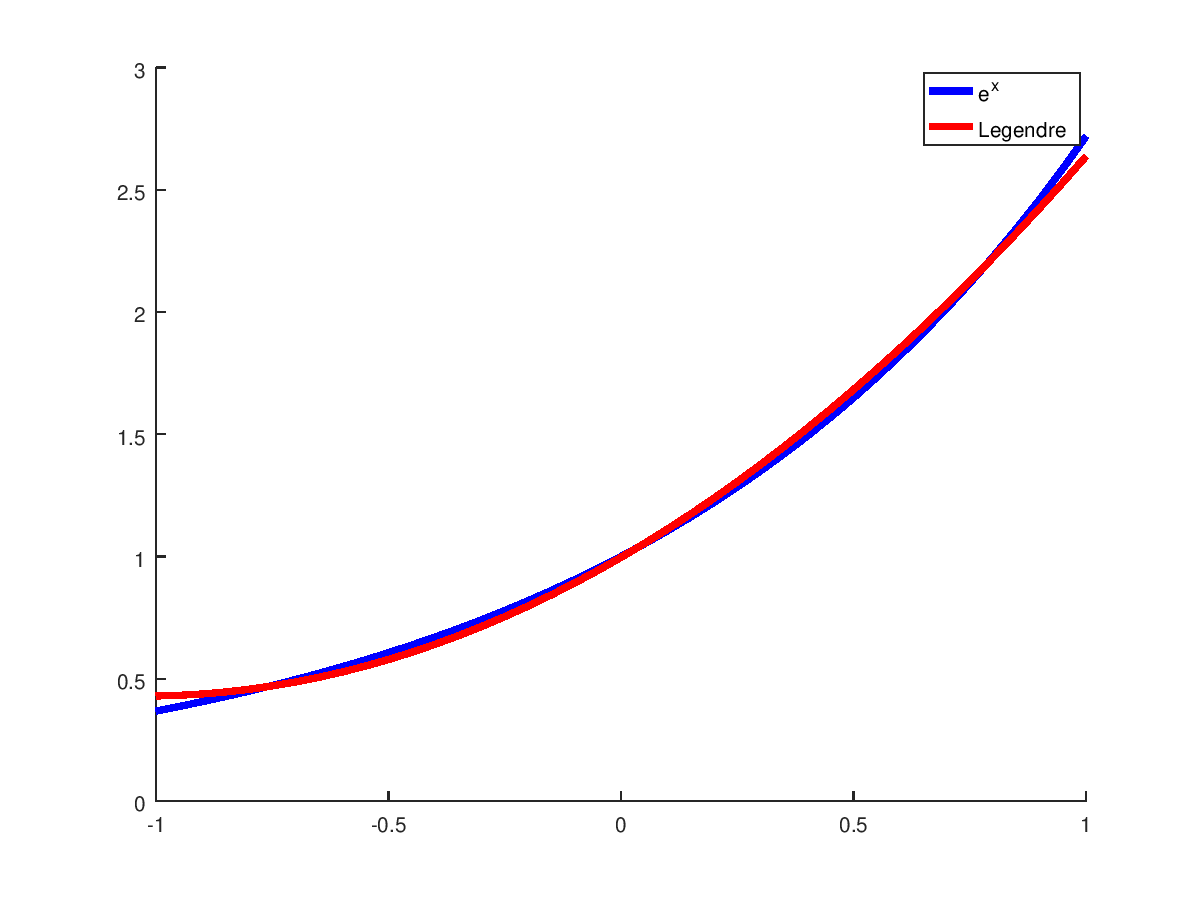
\includegraphics[scale=0.75]{p2b}

%% Problem 3
\problem{} (20 points)

	\begin{enumerate}
		\item Use the zeros of $\overline{T}_4$ to construct an interpolating polynomial of degree
			3 for the following function on the interval $[-1,1]$:
			$$
				f(x) = e^x
			$$
			Find a bound for the maximum error of the approximation.
		\item Repeat (a) on interval $[0, 2]$.
	\end{enumerate}

\solution

	\part

	First, note that we will have 4 zeros of $T_4$ given by $\cos(\frac{2k-1}{2n}\pi)$.
	These are the values $x_0 = \{0.92388, 0.38268, -0.38268, -0.92366\}$.
	Evaluating our function at these points produces $f(x_0) = \{2.51904, 1.46621, 0.68203, 0.39698\}$.
	Next we set up our linear equation to find the coefficients of our polynomial.

	\bigbreak
	\left[\begin{array}{cccc}
		0.92388^3 & 0.92388^2 & 0.92388 & 1 \\
		0.38268^3 & 0.38268^2 & 0.38268 & 1 \\
		-0.38268^3 & -0.38268^2 & -0.38268 & 1 \\
		-0.92388^3 & -0.92388^2 & -0.92388 & 1 \\
	\end{array} \right]
	\left[\begin{array}{c}
		a \\ b \\ c \\ d \\
	\end{array} \right] =
	\left[\begin{array}{c}
		2.51904 \\ 1.46621 \\ 0.68203 \\ 0.39696 \\
	\end{array} \right]

	\bigbreak
	Solving this yields
	\bigbreak
	\left[\begin{array}{c}
		a \\ b \\ c \\ d \\
	\end{array} \right] =
	\left[\begin{array}{c}
		0.17518 \\ 0.54290 \\ 0.99893 \\ 0.99462 \\
	\end{array} \right] \bigbreak
	Which produces the 4th degree polynomial $0.17518x^3 + 0.54290x^2 + 0.99893x + 0.99462$. \\
	To find an upper bound for the error on the bounds I simply need to solve
	$$
		\text{max}_{-1,1}(|0.17518x^3 + 0.54290x^2 + 0.99893x + 0.99462 - e^x|)
	$$
	This occurs at $x=1$ which evaluates to an error of $e - \frac{271163}{100000} \approx 0.00665183$.

	\clearpage
	Once printed out you may not be able to see $e^x$ below the interpolating polynomial,
	clearly this method is doing a pretty decent job of approximating on the given bounds.
	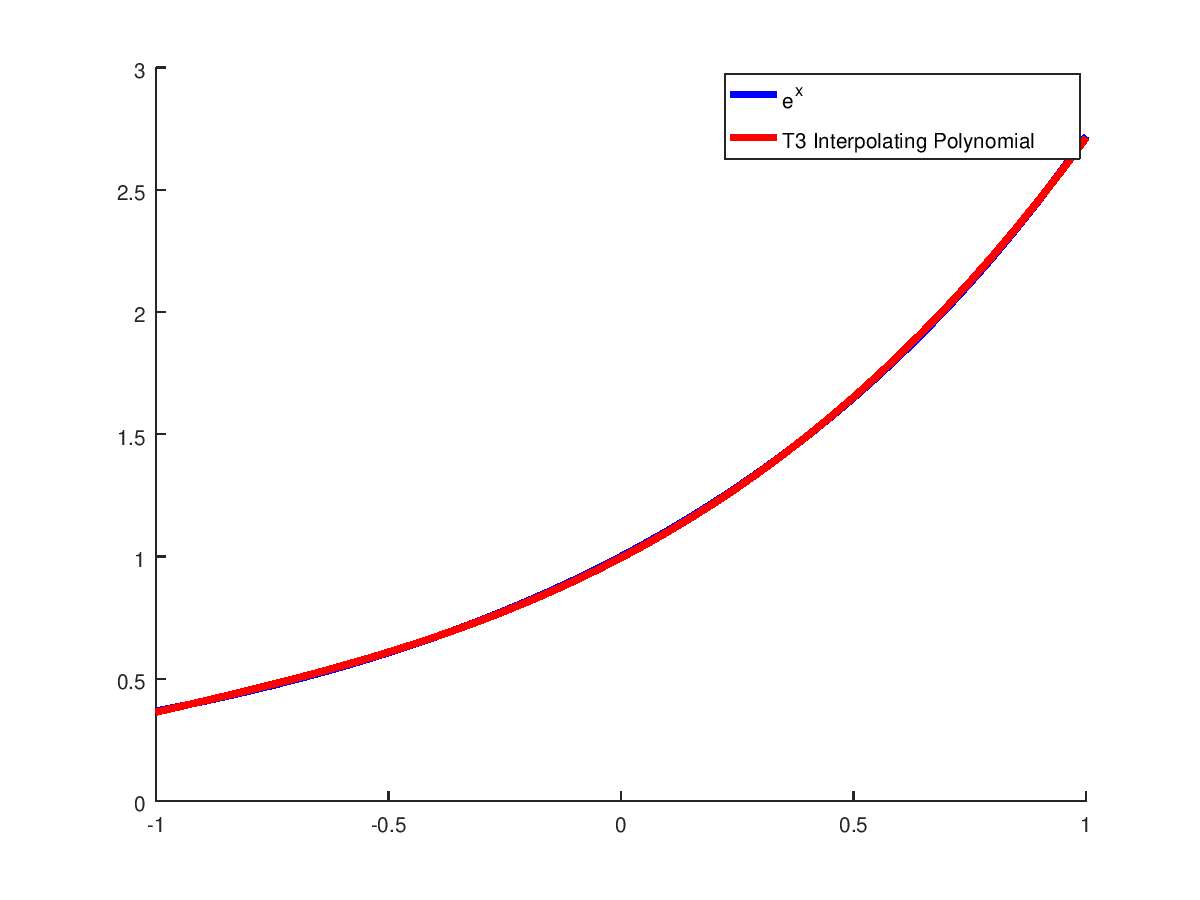
\includegraphics[scale=0.75]{p3}

	\part
	We can follow the same process as part a, but instead use the 4 zeros given by 
	$1 + \cos(\frac{2k-1}{2n}\pi)$. These are the zeros 
	$x_0 = \{1.923880, 1.382683, 0.617317, 0.076120\}$. Evaluating our function at these
	points produces $f(x_0) = \{6.8475, 3.9856, 1.8539, 1.0791\}$. Again, we set up
	and solve our linear equation to find the coefficients of our polynomial.

	\bigbreak
	\left[\begin{array}{cccc}
		1.92388^3 & 1.92388^2 & 1.92388 & 1 \\
		1.38268^3 & 1.38268^2 & 1.38268 & 1 \\
		0.617317^3 & 0.617317^2 & 0.617317 & 1 \\
		0.076120^3 & 0.076120^2 & 0.076120 & 1 \\
	\end{array} \right]
	\left[\begin{array}{c}
		a \\ b \\ c \\ d \\
	\end{array} \right] =
	\left[\begin{array}{c}
		6.8475 \\ 3.9856 \\ 1.8539 \\ 1.0791 \\
	\end{array} \right]

	\bigbreak
	Solving this yields
	\bigbreak
	\left[\begin{array}{c}
		a \\  b \\  c \\ d \\
	\end{array} \right] =
	\left[\begin{array}{c}
		0.476177 \\ 0.047226 \\ 1.192398 \\ 0.987843 \\
	\end{array} \right] \bigbreak

	\bigbreak
	Which gives us the polynomial $0.476177x^3 + 0.047226x + 1.192398x + 0.987843$.
	To find an upper bound for the error on the bounds I simply need to solve
	$$
		\text{max}_{0,2}(|0.476177x^3 + 0.047226x + 1.192398x + 0.987843 - e^x|)
	$$
	This occurs at $x=2$ which evaluates to an error of $e^2 - \frac{1474191}{200000} \approx 0.018101$.
	We can see that as $e^x$ starts to blow up, our polynomial will obviously start to perform worse
	relative to the bounds of part (a).

	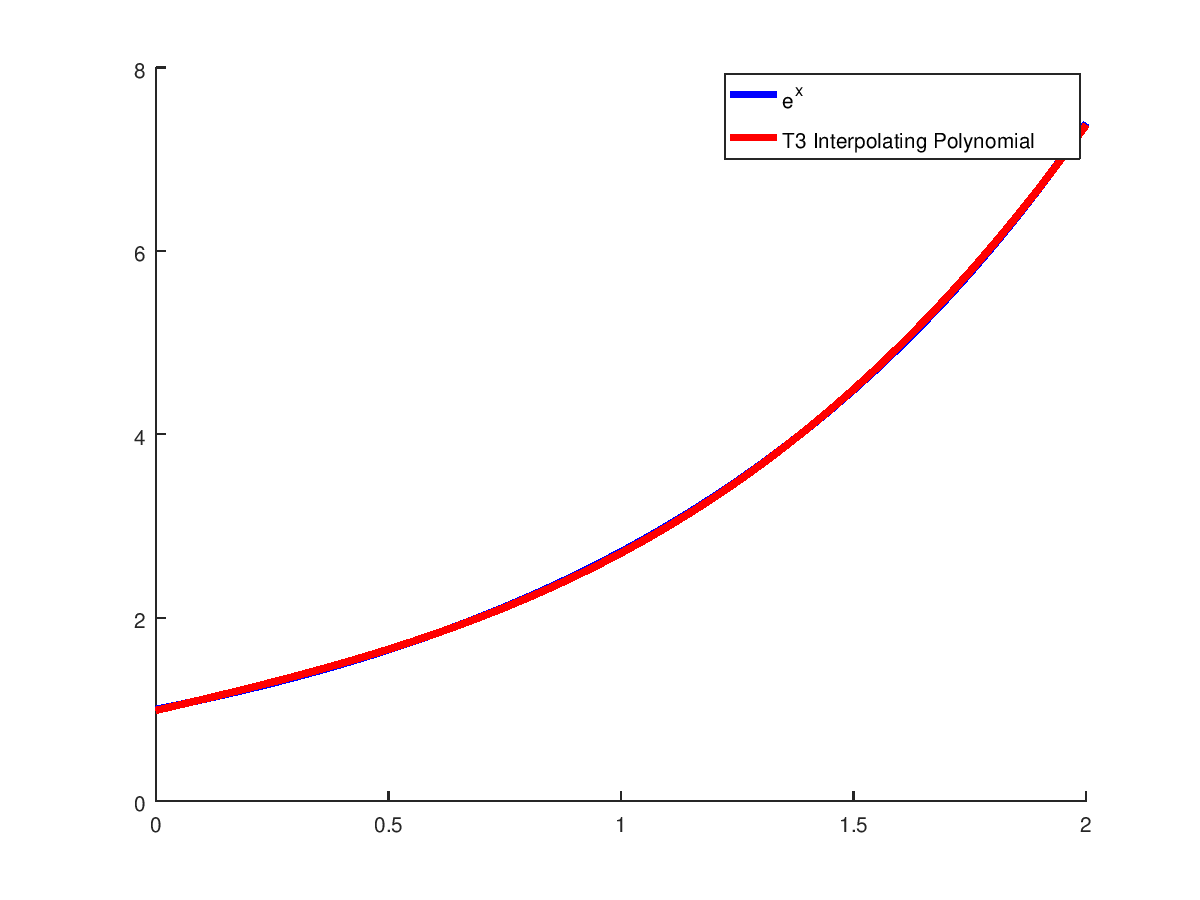
\includegraphics[scale=0.75]{p3b}

%% Problem 4
\problem{} (20 points)
	Find all the Chebyshev rational approximations of degree 2 for $f(x) = e^{-x}$.
	Graph the function and the polynomial. (Use MATLAB routines on classpage)

\solution

	From the sample code posted on the class page we can derive these pretty easily. \\
	As noted in the code there are three possible cases.

	\bigbreak
	\textbf{(n=0, m=2)} \\
	Here we have the vectors $p=[0.79040]$ and $q=[1, 0.88911, 0.19759]$. \\
	Our polynomial then takes the form... \\
	\begin{align*}
		\frac{T_{0,n}(x) p}{T_{0,m}(x) q} &= \frac{0.79040}{1 + 0.88911x + (2x^2-1)0.19759} \\
		&= \frac{0.79040}{0.39518x^2 + 0.8891x + 0.80241}
	\end{align*}
	We can graph this to see how well of an approximation this is. We know from the
	MATLAB code provided on the course page our error is about $0.15604$. \\
	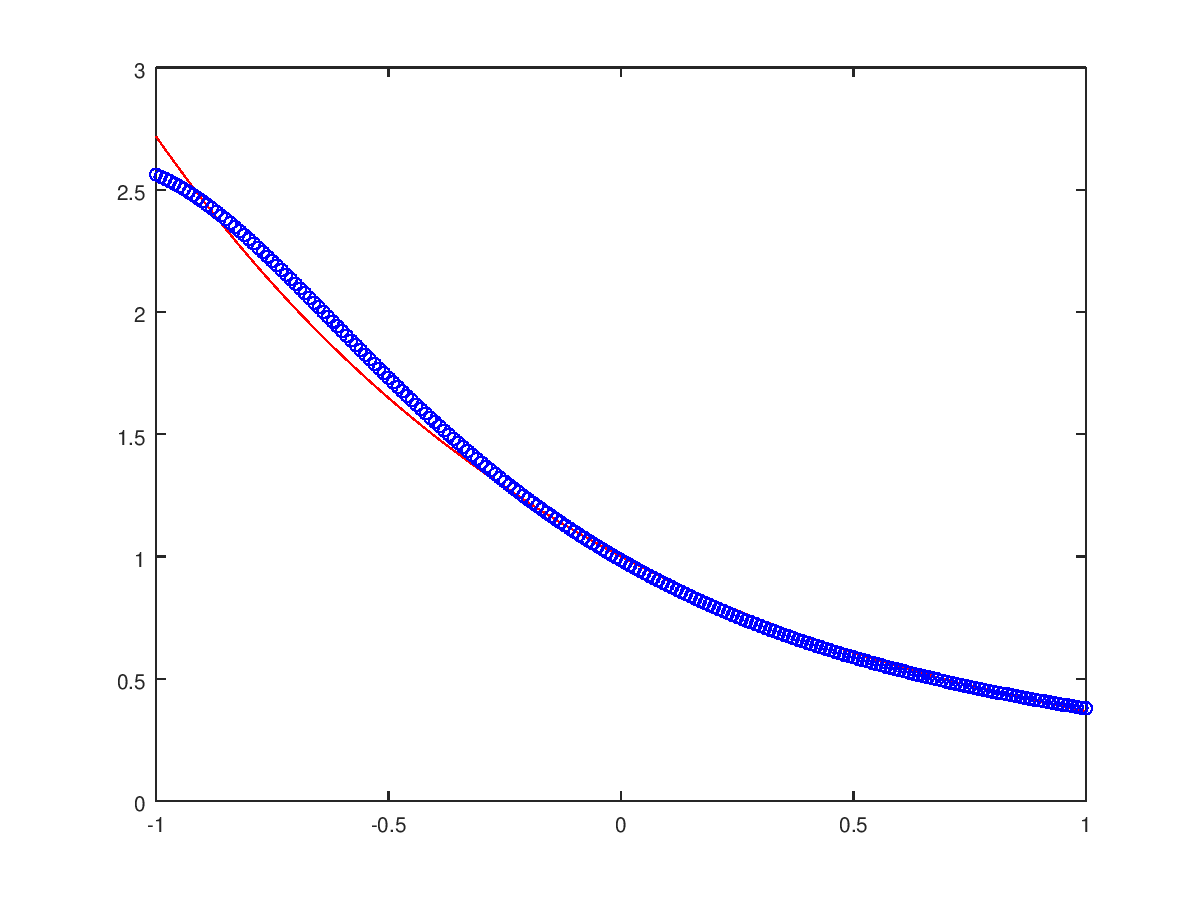
\includegraphics[scale=0.75]{p4a}

	\clearpage
	\textbf{(n=1, m=1)} \\
	Again, using the sample code provided on the class page, we have
	the vectors $p=[1, -0.48232]$ and $q=[1, 0.46626]$. \\
	Our polynomial then takes the form... \\
	\begin{align*}
		\frac{T_{0,n}(x)p}{T_{0,m}(x)q} &= \frac{1 - 0.48232x}{1 + 0.44626x} \\
		&= \frac{4.66276}{x + 2.24085} - 1.0808\\
	\end{align*}
	We can graph this to see how well of an approximation we have. From the MATLAB
	code we can see an error of $0.047232$ a significant improvement over the first case.
	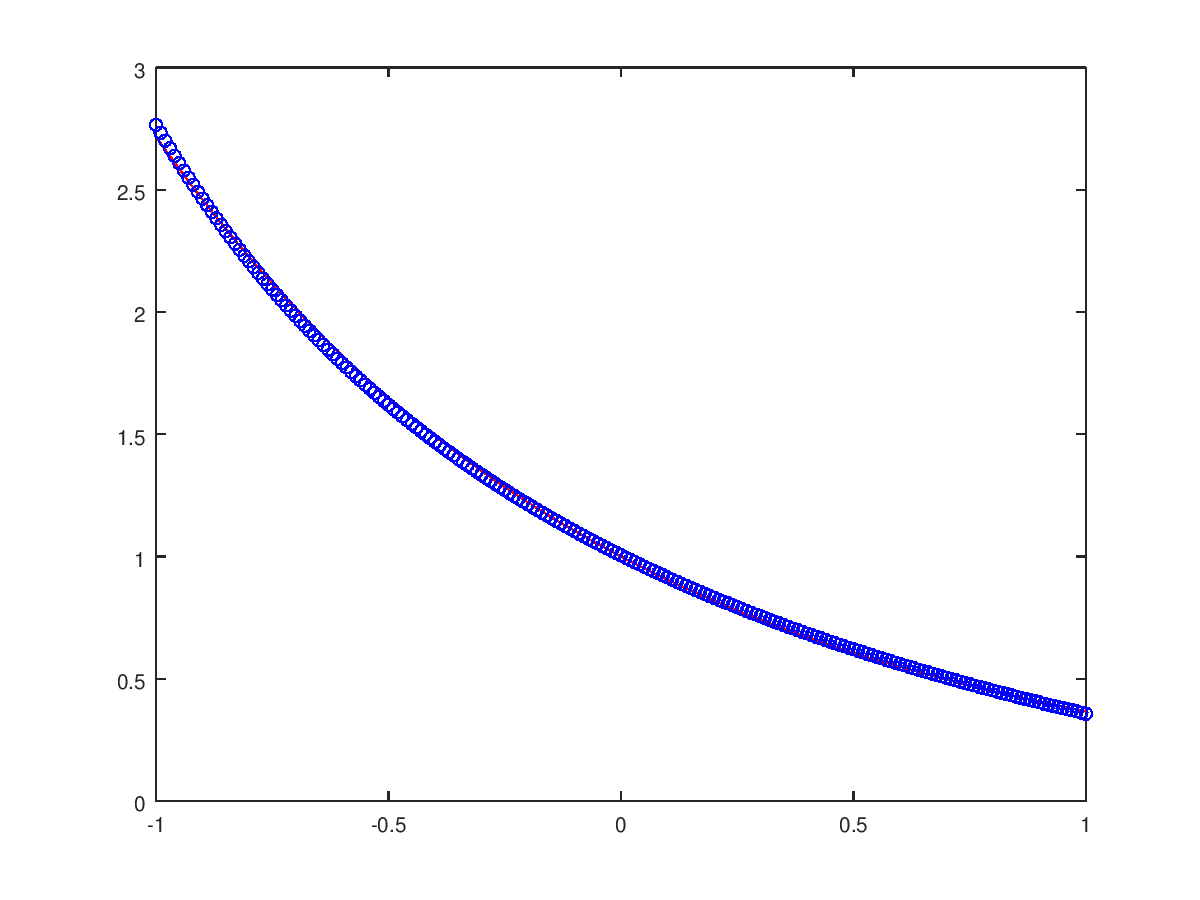
\includegraphics[scale=0.75]{p4b}

	\clearpage
	\textbf{(n=2, m=0)} \\
	In the final case, we have the vectors
	$p=[1.26607, -1.13032, 0.27150]$ and $q=[1]$.
	Giving us the polynomial... \\
	\begin{align*}
		\frac{T_{0,n}p}{T_{0,m}q} &= \frac{1.26607 - 1.13032x + 0.27150(2x^2-1)}{1} \\
		&= 0.543x^2 - 1.13032x + 0.99457 \\
	\end{align*}
	The graph of which is included below, from the MATLAB code we see it has an error
	of $0.050402$, slightly worse than the error of the second case.
	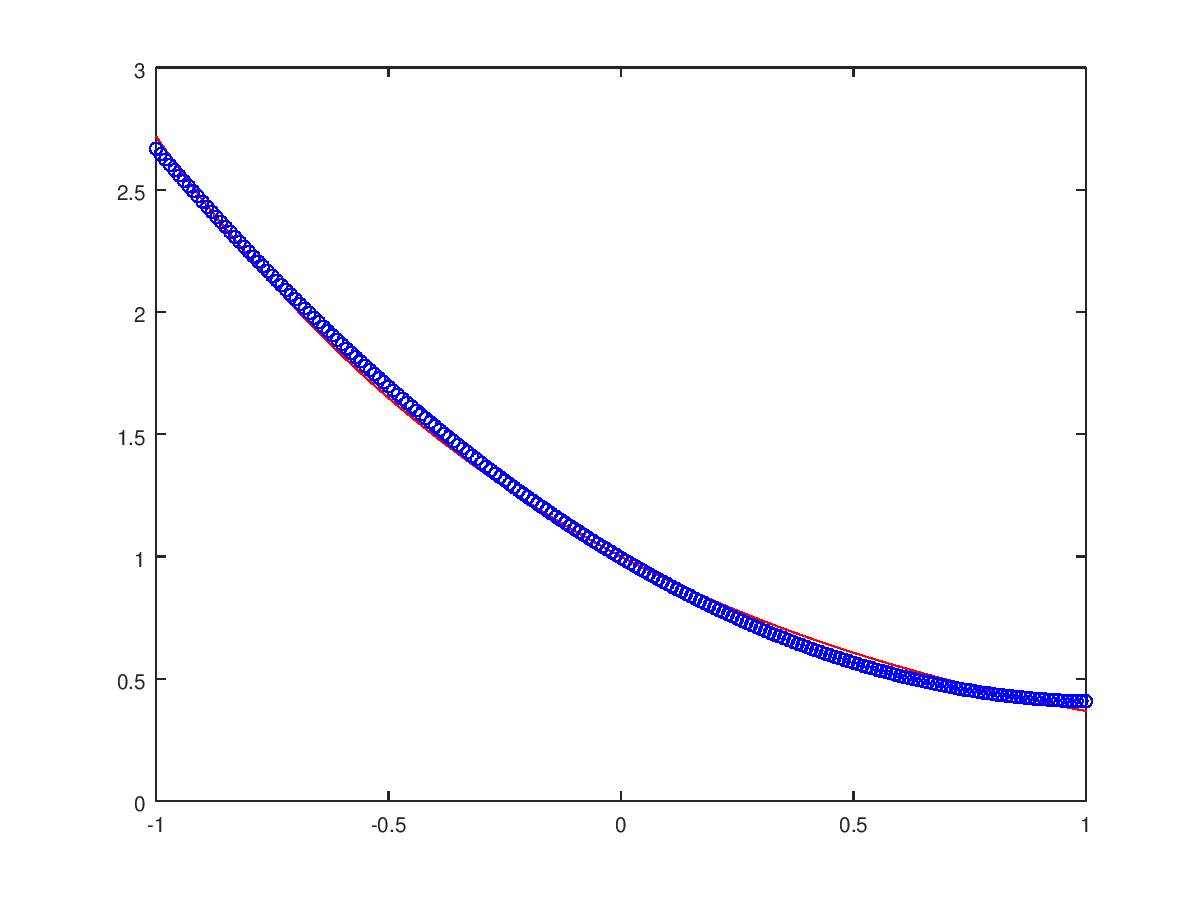
\includegraphics[scale=0.75]{p4c}

%% Problem 5
\problem{} (30 points) (Use MATLAB routines on classpage)

	\begin{enumerate}
		\item Find the continous least squares trigonometric polynomial $S_3(x)$ for
			$f(x) = e^x$ on $[-\pi,\pi]$.
		\item Find the discrete least squares trigonometric polynomials $S_n(x)$ for
			$f(x) = e^x$ on $[-\pi, \pi]$ with $n=3, m=6$.
		\item Find the trigonometric interpolating polynomial $S_n(x)$ for 
			$f(x) = e^x$ on $[-\pi, \pi]$ with $n=8$.
	\end{enumerate}

\solution

	TODO

\end{document}
